\documentclass{article}
\usepackage{amsmath}
\usepackage{empheq}
\usepackage{graphicx}
\usepackage{gvv}
\begin{document}
\title{
\Huge\textbf{Discrete Assignment}\\
\Huge\textbf{EE1205} Signals and Systems\\
\date{}
}
\large\author{Praful Kesavadas\\EE23BTECH11049}
\maketitle

\textbf{Question 11.9.1.2:}
Write the first five terms of the sequence whose $n^{th}$ terms  $x\brak{n} = \frac{n}{n+1}$\\
\textbf{Solution:}
\begin{table}[ht]
  \centering
  \begin{tabular}{|c|c|}
    \hline
    \textbf{Term} & \textbf{Value} \\
    \hline
    $x\brak{n}$ & $\frac{n}{n+1}$$u\brak{n}$ \\
    \hline
  \end{tabular}
  \caption{Input Parameters: General term}
\end{table}\\
Here, Z-transform
\begin{align}
X(z) &= \sum_{i=1}^\infty\ x\brak{n}.z^{-n}\\
&= \sum_{i=1}^\infty \frac{n}{n+1} . z^{-n}\\
&= \sum_{i=1}^\infty u\brak{n}.z^{-n} - \frac{1}{n+1} u\brak{n}.z^{-n}
\end{align}
On solving, 
\begin{align}
Z\{u\brak{n}\} &= \frac{1}{1-z^{-1}}\\
Z\{\frac{-1}{n+1}.u\brak{n}\} &= z\log(1-z^{-1})\\
X(z) &= \frac{1}{1-z^{-1}} + z\log{(1-z^{-1})}\
\end{align}
\begin{figure}[h]
    \centering
    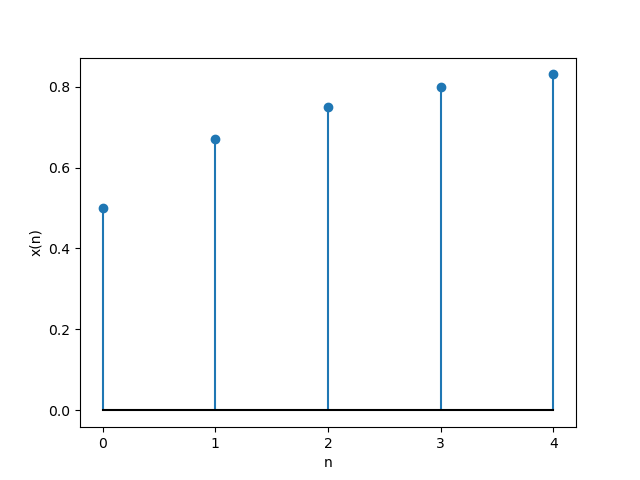
\includegraphics[width=\columnwidth]{figs/graph1.png}
    \caption{Sequence plot generated from Python script}
    \label{fig:sequence-plot}
\end{figure}
\end{document}
